\chapter{Landasan Teori}
\label{sec:landasanteori}

\section{Odoo}
\label{sec:odoo}

Odoo adalah aplikasi \textit{Enterprise Resource Planning} (ERP) open source adalah web aplikasi yang dibangun menggunakan bahasa pemrograman Python, XML, dan JavaScript dan menggunakan PostgreSQL sebagai database management sistemnya.  Odoo merupakan sebuah sistem atau software manajemen open source, yang sangat mudah untuk digunakan. Bentuk dari sistem Odoo ini terdapat berbagai macam, diantaranya adalah berbasis web, desktop serta mobile. Selain itu, software ini memiliki banyak kelebihan seperti didukung oleh banyak komunitas, modul yang lengkap dan terintegrasi, pemasangan yang mudah, dan juga biaya yang terjangkau. Aplikasi bisnis yang terintegrasi dalam Odoo berbentuk modul-modul yang siap untuk diunduh dan digunakan dan sebagian besar bisa didapatkan secara gratis \cite{suminten}.

\subsection{Struktur Direktori}
\label{sec:strukturDirektori}

\subsection{Instalasi}
\label{sec:instalasi}
Pada skripsi ini Odoo akan dinstalasi menggunakan cara \textit{Source Install}, proses instalasi ini bukan hanya sekedar install odoo dan menggunakannya langsung dari sumber website Odoo. Proses instalasi ini lebih nyaman digunakan oleh penulis karena untuk mengembangkan modul akan lebih mudah untuk diakses dibandingkan menggunakan instalasi yang sudah paket.
Dalam proses penggunaan Odoo, akan lebih mudah untuk menjalankan dan menghentikan Odoo, sehingga terlihat lebih flexibel dibandingkan menggunakan instalasi yang sudah satu paket dan juga memungkinkan pengaturan menggunakan baris perintah, tanpa harus mengubah file konfigurasi pada Odoo. Secara tidak langsung, proses intalasi ini memberikan kontrol yang lebih besar atas pengaturan sistem dan memungkinkan untuk lebih mudah menyimpan dan menjalankan beberapa versi Odoo secara bersamaan. \footnote{Instalasi Odoo \url{https://www.odoo.com/documentation/16.0/administration/install/install.html}} Terdapat beberapa cara mengenai cara untuk melakukan instalasi Odoo 16, yaitu:
\begin{enumerate}
	\item Online \\
	Instalasi secara online adalah cara termudah untuk menggunakan Odoo dalam membangun sistem produksi.
	\item Package installer \\
	Instalasi secara \textit{package installer} adalah cara yang sempurna untuk menguji Odoo, mengembangkan modul, dan dapat digunakan untuk penggunaan produksi jangka panjang dengan intalasi tambahan dan \textit{maintenance} tambahan.
	\item Install source \\
	Instalasi secara \textit{install source} adalah cara install odoo dengan memberikan fleksibilitas yang lebih besar, contohnya adalah memungkinkan beberapa versi Odoo berjalan di sistem yang sama, baik untuk mengembangkan modul. Instalasi source ini adalah cara install Odoo yang akan digunakan pada skripsi ini.
	\item Docker \\
	Instalasi Docker dapat digunakan untuk instalasi Odoo karena pengembangan aplikasi yang cepat, mudah, dan portabel.
\end{enumerate}

Pada proses instalasi secara source, terdapat dua cara untuk mengunduh kode Odoo, yaitu melalui arsip zip atau menggunakan git. Dalam penulisan skripsi ini akan dilakukan instalasi Odoo menggunakan git dalam mendapatkan kode Odoo. Tahapan pertama dalam instalasi ini adalah Git harus sudah terinstal di perangkat yang akan digunakan, dan developer harus memiliki pengetahuan dasar dalam proses penggunaan Git. Selanjutnya, untuk mengkloning repositori Git, developer harus memilih salah satu cara antara mengkloning dengan HTTPS atau SSH.

\begin{figure}[H]
	\centering
	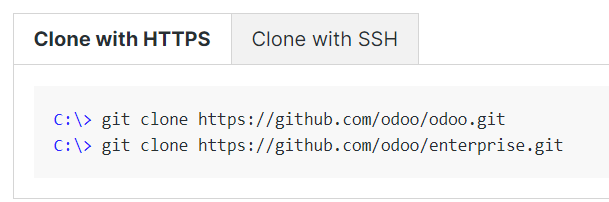
\includegraphics[scale=0.7]{Gambar/clone.png}
	\caption{Contoh Intalasi Source menggunakan Git} 
	\label{fig:clonegit}
\end{figure}

Tahap selanjutnya adalah mempersiapkan Python, sistem Odoo membutuhkan minimal versi 3.7 atau lebih, apabila Python sudah pernah diinstal, maka harus dilakukan pemerikasaan apakah Python sudah menggunakan versi 3.7 atau belum, karena versi dibawah 3.7 tidak cocok untuk instalasi Odoo. Cara yang dapat dilakukan untuk melihat versi Python dapat menggunakan cara sebagai berikut melalui \textit{command prompt} (CMD).

\begin{figure}[H]
	\centering
	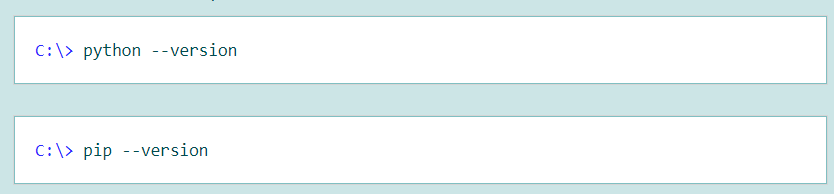
\includegraphics[scale=0.7]{Gambar/python.png}
	\caption{Contoh Melihat Versi Python dan Pip} 
	\label{fig:pip}
\end{figure}

Tahap selanjutnya adalah mempersiapkan PostgreSQL. Odoo menggunakan PostgreSQL sebagai sistem manajemen basis data. Pengguna dapat mengunduh dan instal PostgreSQL minimal versi 12.0 atau yang lebih terbaru. Pada proses intalasi PostgreSQL, pengaturan awal pengguna PostgreSQL adalah postgres, namun Odoo menyarankan untuk tidak menghubungkan database ke postgres, sehingga pengguna diharuskan untuk membuat user atau role baru di PostgreSQL. Berikut tahapan yang harus dilakukan ketika akan melakukan instalasi PostgreSQL:

\begin{enumerate}
	\item Tambahkan direktori bin PostgreSQL (secara pengaturan awal tersimpan di C:-Program Files-PostgreSQL-<version>-bin) ke PATH perangkat yang digunakan. Pada penulisan skripsi ini, PostgreSQL yang digunakan adalah versi 15, sehingga penulisan pada path adalah (C:-Program Files-PostgreSQL-15-bin).
	\item Buat baru nama pengguna postgres dengan kata sandi melalui pgAdmin GUI.
		\begin{itemize}
			\item Buka program pgAdmin.
			\item Klik dua kali pada bagian menu server untuk membuat koneksi.
			\item Pilih bagian menu Objek lalu buat nama untuk login atau role.
			\item Input nama di kolom nama (misalkan: odoo).
			\item Pilih bagian \textit{definition} lalu input password.
			\item Pilih bagian \textit{privileges} lalu pilih bagian dapat login dan buat database.
		\end{itemize}
\end{enumerate}

\begin{figure}[H]
	\centering
	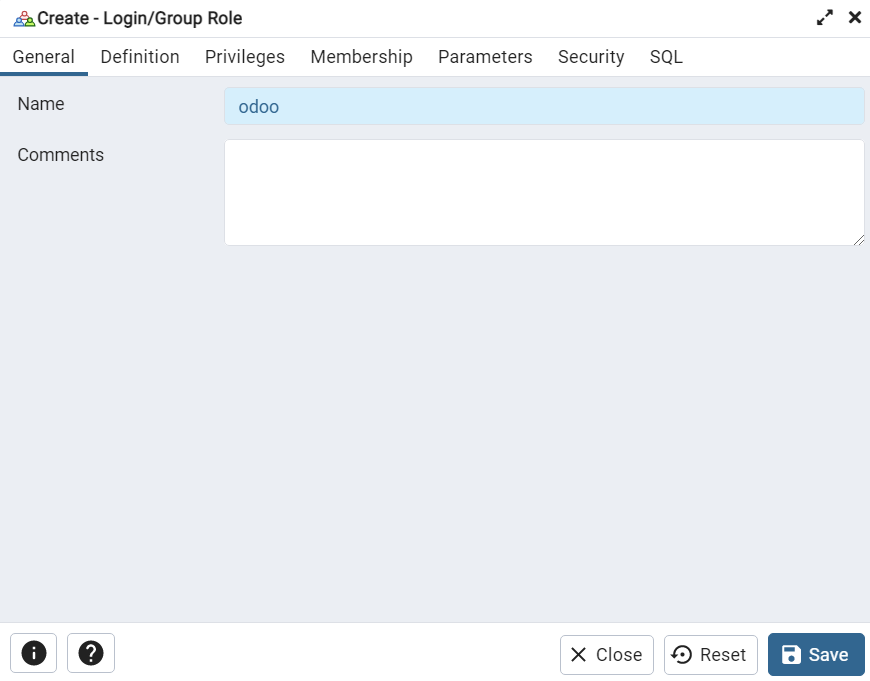
\includegraphics[scale=0.7]{Gambar/psql.png}
	\caption{Contoh Membuat Database pada PostgreSQL} 
	\label{fig:psql}
\end{figure}

Tahapan selanjutnya yang perlu dilakukan dalam instalasi Odoo adalah melakukan beberapa instalasi tambahan. Sebelum proses ini dilakukan, pengguna harus mengunduh dan menginstal \textit{Build Tools for Visual Studio}, lalu pilih C++ build tools pada bagian tab Workloads dan lakukan proses instalasi. Setelah proses ini dilakukan, pengguna harus membuka \textit{command prompt} (CMD) dan melakukan beberapa proses seperti pada gambar berikut:

\begin{figure}[H]
	\centering
	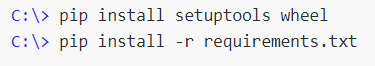
\includegraphics[scale=1]{Gambar/setupOdoo.png}
	\caption{Contoh Perintah untuk Melakukan Proses Instalasi Tambahan} 
	\label{fig:setupOdoo}
\end{figure}

Tahapan terakhir yaitu proses menjalankan Odoo, pada penulisan skripsi ini, penulis menggunakan aplikasi PyCharm, gunakan aplikasi ini untuk membuka folder yang sudah berhasil di clone lalu membukanya melalui PyCharm, setelah itu lakukan beberapa perubahan pada environment, sehingga server Odoo dapat dijalankan. Berikut contoh perubahan pada environment pada PyCharm:

\begin{figure}[H]
	\centering
	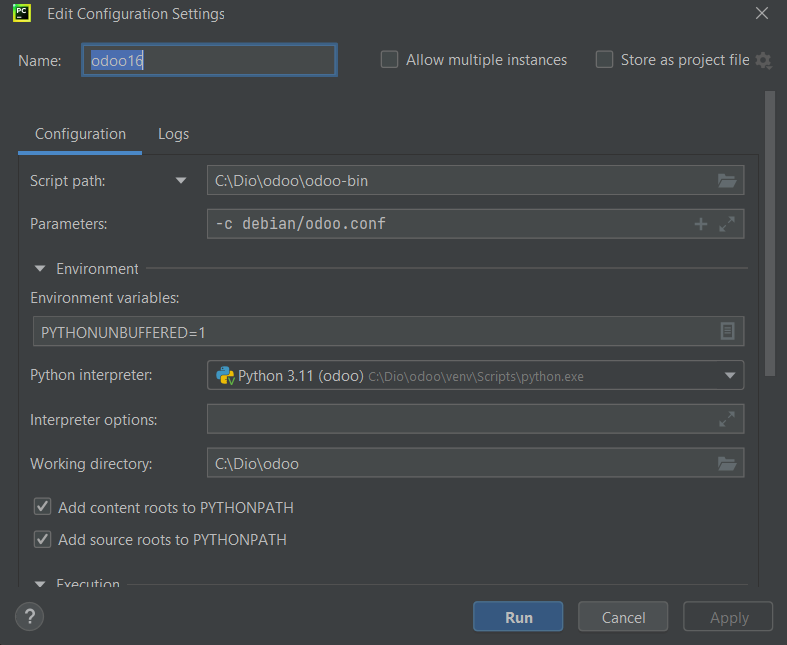
\includegraphics[scale=0.7]{Gambar/pycharm.png}
	\caption{Contoh Perubahan Pengaturan pada PyCharm} 
	\label{fig:pycharm}
\end{figure}

Setelah server berhasil dijalankan (log INFO odoo.modules.loading: Modul sedang diproses), secara pengaturan awal, halaman untuk membuka website awal Odoo adalah \url{http://localhost:8069} yang dilakukan di browser web dan masuk dengan akun admin.

\begin{figure}[H]
	\centering
	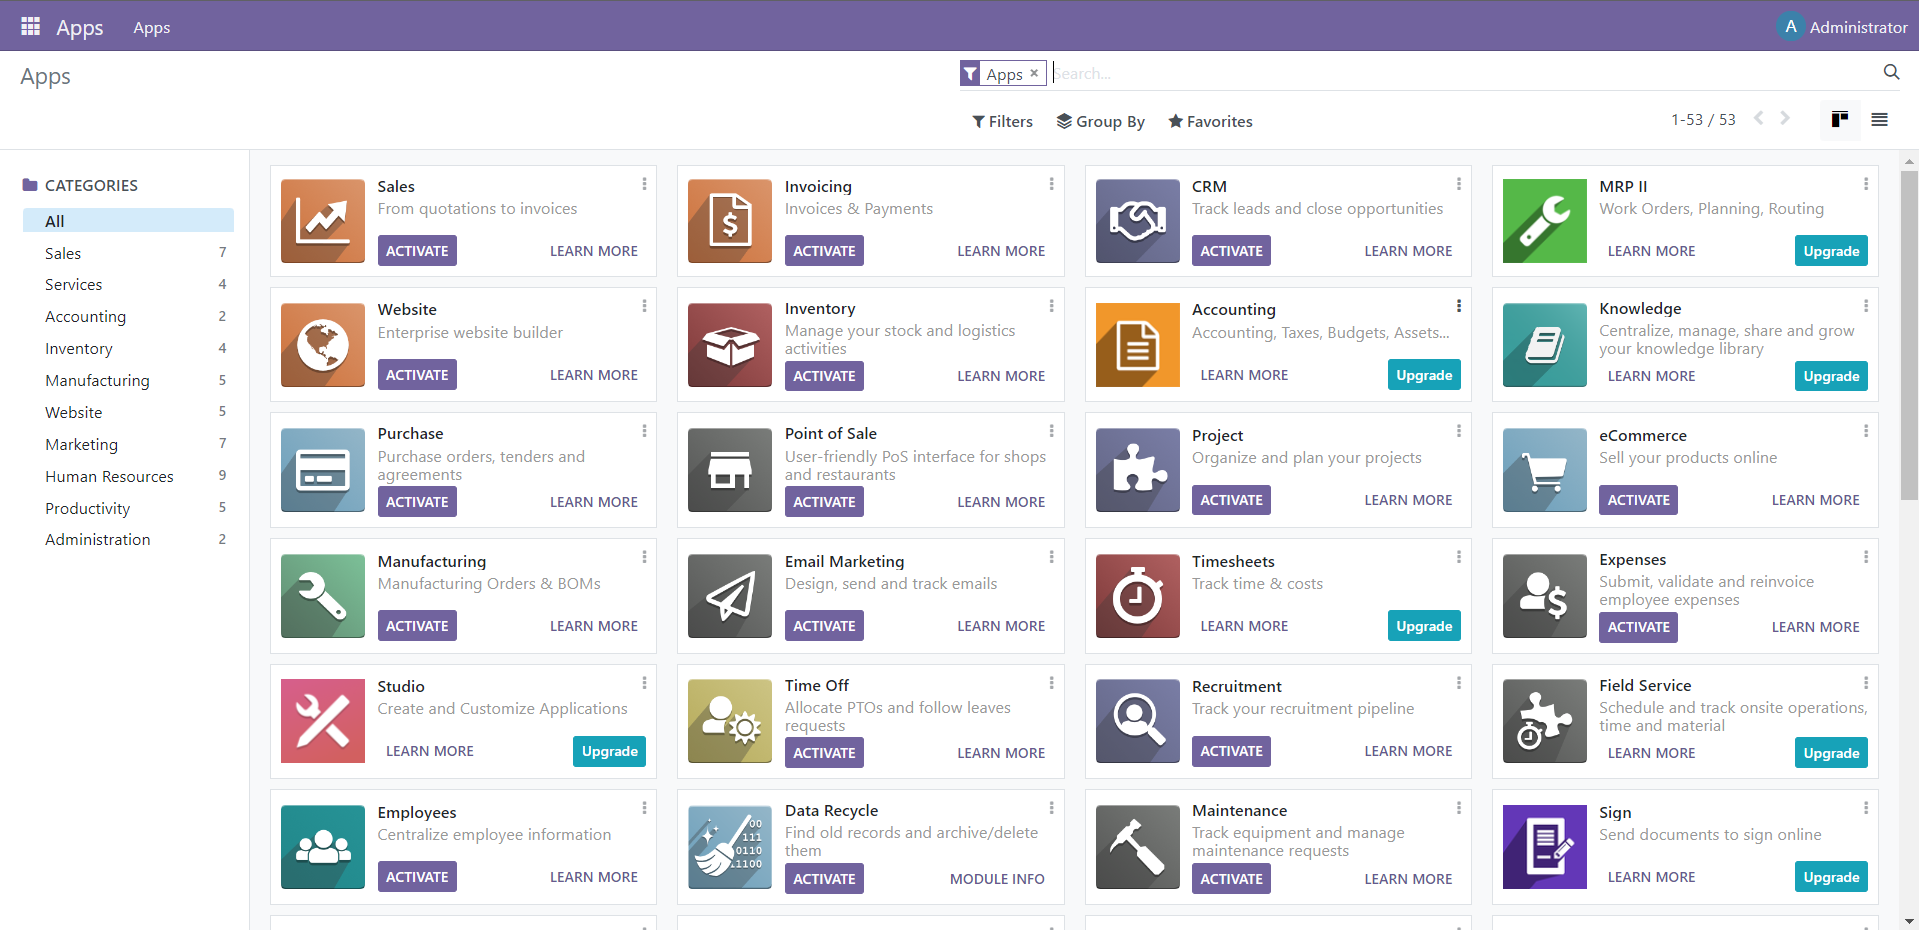
\includegraphics[scale=0.4]{Gambar/halamanOdoo.png}
	\caption{Contoh Halaman Odoo} 
	\label{fig:halamanOdoo}
\end{figure}

\section{Sistem Informasi Manajemen Umat (SIMU)}
\label{sec:simu}
Sistem Informasi Manajemen Umat (SIMU) adalah aplikasi milik Keuskupan Bandung, aplikasi ini bertujuan untuk mencatat data umat dan dinamikanya (contohnya adalah sakramen). Keuskupan Bandung memiliki sekitar 108.000 umat, plus umat Sibolga. Cara kerja sistem ini adalah apabila terdapat ada umat baru yang sebelumnya tidak tercatat di SIMU, berikan print-out dari Formulir Data Umat kepada yang bersangkutan. Jika keluarga juga belum tercatat di SIMU, berikan pula print-out dari Formulir Keluarga Katolik / Rumah Tangga Katolik untuk diisi. Formulir ini biasanya dimiliki oleh paroki masing-masing. Jika tidak tersedia, bisa menghubungi admin keuskupan untuk mendapatkannya.


\section{Design untuk Aplikasi Mobile}
\label{sec:designMobility}
Perangkat seluler (smartphone), tablet, perangkat yang dapat dikenakan, perangkat game genggam telah menjadi umum di dunia komputasi. Desain seluler mencakup aktivitas teknis dan nonteknis yang meliputi beberapa hal, yaitu menetapkan tampilan dan nuansa aplikasi seluler (termasuk aplikasi seluler, WebApps, realitas virtual (VR), dan game), membuat tata letak estetika antarmuka pengguna, menetapkan ritme interaksi pengguna, mendefinisikan struktur arsitektur keseluruhan, mengembangkan konten dan fungsionalitas yang berada di dalam arsitektur, dan merencanakan navigasi yang terjadi di dalam produk seluler. 

Desain seluler biasa dilakukan oleh software engineers, graphic designers, content developers, security specialists, dan semua tim yang tergabung dalam pembuatan model design. Desain sangatlah penting karena memungkinkan suatu model yang dibuat dapat meningkat nilai kualitasnya. Salah satu contohnya adalah website. 

Website adalah sekumpulan halaman yang terdiri dari beberapa laman yang berisi informasi dalam bentuk data digital baik berupa text, gambar, video, audio, dan animasi lainnya yang disediakan melalui jalur koneksi internet. Untuk membangun sebuah halaman website dibutuhkan sebuah bahasa pemrograman yang lebih dikenal dengan sebutan web scripting. 


\subsection{QR Code}
QR Code, kependekan dari Quick Response Code, merupakan gambar dua dimensi yang memiliki kemampuan untuk menyimpan data. QR Code biasa digunakan untuk menyimpan data berupa teks, baik itu numerik, alfanumerik, maupun kode biner. QR Code banyak digunakan untuk keperluan komersil biasanya berisi link url ke alamat tertentu atau sekedar teks berisi iklan, promosi, dan lain-lain. QR Code adalah image dua dimensi yang merepresentasikan
suatu data, terutama data berbentuk teks. QR Code merupakan evolusi dari barcode yang awalnya satu dimensi menjadi dua dimensi. QR Code memiliki kemampuan menyimpan data yang
lebih jauh besar daripada barcode.